%To do: Fix all previous notes

\documentclass{article}
\usepackage[margin=1in]{geometry}
\usepackage{amsmath, amssymb, amsthm}
\usepackage{enumitem}


\usepackage{tikz}
\usepackage{xcolor}
\usepackage{xcolor}
\usetikzlibrary{calc,trees,positioning,arrows,fit,shapes,calc}

%Formatting and Spacing
\setitemize[1]{noitemsep, parsep = 5pt, topsep = 5pt}
\setenumerate[1]{label = (\alph*), parsep = 1pt, topsep = 5pt}
\setlength\parindent{0pt}
\linespread{1.1}

%Custom Title Fields
\newcommand{\lectTitle}{Lecture 6 Notes}
\newcommand{\lectTime}{January 31, 2022}
\newcommand{\lectClass}{Honors Discrete Mathematics}
\newcommand{\lectClassInstructor}{Tillson Galloway}
\newcommand{\lectSection}{Spring 2022}
\newcommand{\lectAuthorName}{Gerandy Brito \& Sarthak Mohanty}

%Headers and Footers
\usepackage{fancyhdr}
\usepackage{extramarks}
\pagestyle{fancy}
\lhead{\lectTime}
\chead{\lectClass \ (\lectClassInstructor)}
\rhead{\lectTitle}
\cfoot{\thepage}
\renewcommand\headrulewidth{0.4pt}
\renewcommand\footrulewidth{0.4pt}

\title{
    \vspace{2in}
    \textbf{\lectClass:\\ \lectTitle}\\
    \vspace{0.1in}\large{\textit{\lectClassInstructor\ \lectSection}}
    \vspace{3in}
    \author{\textbf{\lectAuthorName}}
    \date{}
}

\begin{document}

\maketitle
\pagebreak

\section*{Relations}

    Recall the definition of a relation:
    
    \vspace{1.5mm}
    \textbf{Definition} a \textit{relation} is a subset of the Cartesian product $A\times B$.
    
    \vspace{1.5mm}
    We denote relations by $\mathcal{R}$. We write $a\mathcal{R} b$ to indicate that $(a,b)\in \mathcal{R}$ (i.e.: in the subset denoted by $\mathcal{R}$). When $A=B$ we said that $\mathcal{R}$ is a relation on $A$.\\
    
    Let $\mathcal{R}_1, \dots, \mathcal{R}_4$ be a relation on $A = \{1, 2, 3, 4\}$.
    \begin{itemize}
        \item $\mathcal{R}_1 = \{(a, b) \mid a \le b)\}$
        \item $\mathcal{R}_2 = \{(a, b) \mid a = b)\}$
        \item $\mathcal{R}_3 = \{(a, b) \mid a+b \le 2022)\}$
        \item $\mathcal{R}_4 = \{(a, b) \mid a \text{ divides } b\}$
    \end{itemize}
    Create bijective (bean diagram) graph in tikz.
    
    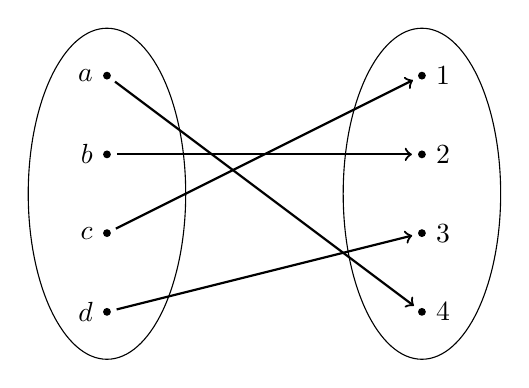
\begin{tikzpicture}[ele/.style={fill=black,circle,minimum width=.8pt,inner sep=1pt},every fit/.style={ellipse,draw,inner sep=-2pt}]
      \node[ele,label=left:$a$] (a1) at (0,4) {};    
      \node[ele,label=left:$b$] (a2) at (0,3) {};    
      \node[ele,label=left:$c$] (a3) at (0,2) {};
      \node[ele,label=left:$d$] (a4) at (0,1) {};
    
      \node[ele,,label=right:$1$] (b1) at (4,4) {};
      \node[ele,,label=right:$2$] (b2) at (4,3) {};
      \node[ele,,label=right:$3$] (b3) at (4,2) {};
      \node[ele,,label=right:$4$] (b4) at (4,1) {};
    
      \node[draw,fit= (a1) (a2) (a3) (a4),minimum width=2cm] {} ;
      \node[draw,fit= (b1) (b2) (b3) (b4),minimum width=2cm] {} ;  
      \draw[->,thick,shorten <=2pt,shorten >=2pt] (a1) -- (b4);
      \draw[->,thick,shorten <=2pt,shorten >=2] (a2) -- (b2);
      \draw[->,thick,shorten <=2pt,shorten >=2] (a3) -- (b1);
      \draw[->,thick,shorten <=2pt,shorten >=2] (a4) -- (b3);
     \end{tikzpicture}
    So why relations? They are more general and allow us to study more complex sets. Elaborate. \\
    
\subsection*{Properties}
    
    \begin{itemize}
        \item \underline{Reflexive:} $(\forall a \in A)(a\mathcal{R}a)$
        \item \underline{Symmetric:} $(\forall a, b \in A)(a\mathcal{R}b \iff b\mathcal{R}a)$
        \item \underline{Antisymmetric:} $(\forall a, b\in A)(a\mathcal{R}b \wedge b\mathcal{R}a \rightarrow a=b)$
        \item \underline{Transitive:} $(\forall a, b, c\in A)(a\mathcal{R}b \wedge b\mathcal{R}c \rightarrow a\mathcal{R}c)$
    \end{itemize}
    Create visualization graph in tikz.
    
    We checked these properties for $R_{2}$ and $R_{3}$. $\mathcal{R}_{2}$ was reflexive, symmetric, and transitivity. $\mathcal{R}_{3}$ was symmetric and transitive?
    
\section*{Functions}
    Last lecture, we informally covered the meaning of a function. With our new knowledge of relations, we now have the tools to formally define them.
    
    \vspace{1.5mm}
    \textbf{Definition}
    A function is a relation on $A\times B$ such that 
    $$(\forall a \in A)(\exists! b \in B)(a\mathcal{R}b).$$
    
    By the way, the propositional symbol $\exists!$ means ``there exists only one".
    
    Often we are presented with functions describing the unique element $b$ for each $a$. In this case we use $f$ to denote the function and write $F A \mapsto B$ or $b=f(a)$. \\
    
    A function $f$ is a way to associate each item in a set to an element in another set. \\
    
    
    Notation:\\
    Usually, we write functions abstractly as $F: A \mapsto B$.
    
    $A$ is called the domain. $B$ is called codomain. The range of $f$ is the set of all $b\in B$ for which there is at least one $a\in A$ satisfying $f(a)=b$. 
    
    To do: think of the representation using relations.
    
    
\subsection*{Classes of Functions}
    \begin{enumerate}
        \item A function is \textit{surjective} (or onto) if every element in $B$ is associated with at least one element in $A$. In other terms, the range is equal to the codomain. \\
        \item A function is \textit{injective} (or one-to-one) if no two elements $b_1, b_2 \in B$ such that $b_1 \neq b_2$ but $f(b_1) = f(b_2)$. In other terms, no two distinct elements in $B$ associate to the same $a \in A$. \\
        \item A function is \textit{bijective} if it is surjective and injective.
    \end{enumerate}
    
    Examples:
    What are the domain and codomain of the following functions. Also determine whether the following functions are surjective, injective, or both (bijective).
    \begin{itemize}
        \item $f$ assigns to each student in the class its height in cm.
        \item $f(x) = x+1$ from $\mathbb{N}$ to itself, then from $\mathbb{Z}$ to itself.
        \item $f$ assigns to each bit string of length two or more its last two bits.
        \item $f$ assigns to each real number the largest integer less or equal than the number
    \end{itemize}
    
    Solutions:
    \begin{itemize}
        \item Domain: Students, Codomain: $\mathbb{R}^{+}$. Neither injective nor surjective.
        \item This function is only injective when mapping from $\mathbb{N}$ to itself, as $f(x) = 1$ cannot be reached by any $x \in \mathbb{N}$. However, when mapping from $\mathbb{Z}$ to itself, this function becomes bijective.
        \item D: bitstrings length greater than 2, C: bitstrings length 2. Surjective
        \item $\mathbb{R} \rightarrow \mathbb{Z}$, Surjective
    \end{itemize}
    
    To do:  discuss what it means to be one-to-one, onto, in the language of relations.
    
    %only work if $A=B$! Help then visualize what it means to be reflexive (the main diagonal is in $\mathcal{R}$); symmetric ($\mathcal{R}$ is symmetric with respect to the main diagonal); and antisymmetric  (there are no symmetric points!)
    
    % Write the definitions. Mention that, in practice, we get functions not as relations and work directly with the $f$ description. Now give then the general strategy to prove a function is one-to-one:
    $$f\text{ is one-to-one if } f(x) = f(y) \rightarrow x = y$$
    
    and onto
    $$f\text{ is onto if } (\forall b\in B)(\exists a\in A) (f(a)=b)$$
    To do: give examples to prove this

\subsection*{To do: Briefly cover Inverses}

\section{Equivalence Relations}
    
    {\bf Def:} A relation is said to be an equivalence relation if it is reflexive, symmetric, and transitive. \\
    
    Example: Show that the relation on the real numbers defined as $a\mathcal{R}b \leftrightarrow a-b\in \mathbb{Z}$ is an equivalence relation.\\
    
    \vspace{1.5mm}
    Solution: 
    Reflexive: $a = b$, then $a \mathcal{R} a$ because $a - a = 0$. \\
    Symmetry: $a - b = -(b - a)$. Assume $a \mathcal{R} b$. Then $b \mathcal{R} a$ because $-b + a \rightarrow a - b$? \\
    Transitivity: Assume $a \mathcal{R} b$ and $b \mathcal{R} c$, WTS $a \mathcal{R} c$ $a - b = d, d \in \mathbb{Z}$. $b - c = e, e \in \mathbb{Z}$. $d + e = (a - b) + (b - c) = a- c)$.
    
    \textbf{Definition}
    Given a set $A$ and an equivalence relation on it, the equivalence classes are the sets
    $$[a]_{\mathcal{R}}=\{x\in A~|~a\mathcal{R} x\}$$
    
    \textbf{Theorem} Let $A$ be a set and $\mathcal{R}$ an equivalence relation on it. The following are equivalent:
    \begin{itemize}
        \item[(i)] $a\mathcal{R}b$.
        \item[(ii)] $[a]_{\mathcal{R}}=[b]_{\mathcal{R}}$.
        \item[(iii)] $[a]_{\mathcal{R}}\cap [b]_{\mathcal{R}}\neq \emptyset$.
    \end{itemize}
    
    \textbf{Proof} 
    \begin{itemize}
        \item (i) to (ii): Suppose $a \mathcal{R} b$. Let $c \in [a]_{\mathcal{R}}$. Then $a \mathcal{R} c$. By the symmetry property of equivalence relations. Since $a \mathcal{R} b$ and $a \mathcal{R} c$, we have $b \mathcal{R} a$ and $a \mathcal{R} c$, so $b \mathcal{R} c$.
        \item (ii) to (iii): Suppose $[a]_{\mathcal{R}}=[b]_{\mathcal{R}}$. If $a = b \rightarrow = a \mathcal{R} a$ by reflexivity.
        \item (iii) to (i) Assume $[a]_{\mathcal{R}} \cup [b]_{\mathcal{R}} \ne \emptyset$. Then there exists some $c$ such that $c \in [a]_{\mathcal{R}}$ and $c \in [b]_{\mathcal{R}}$. Then $a \mathcal{R} c$ and $b \mathcal{R} c$. Then by symmetry, we have $c \mathcal{R} b$. By transitivity, we conclude that $a \mathcal{R} b$, as desired.
    \end{itemize}
    
    To do: redefine
    \vspace{1.5mm}
    \textbf{Definition}: $P$ is a partitioning of $A_{i}$ for all $i$ iff $\bigcup_{i = 1}^{k} P_{i} = A$, where each $P_{i}$ is disjoint.
    
     Why is every element in a class? Ans: because of the reflexive property. Why it is a partition? Because of facts (ii) and (iii) of the Theorem.

\section*{Post Lecture}

\subsection*{Question 1}
    Al and Bob play a game. They have the numbers $1,2,\dots, 9$ written on cards face up. Players alternate taking any card. The first player to have exactly 3 cards whose sum is 15 wins. Determine which player, if any, has a winning strategy.
    
    \vspace{1.5mm}{\small \textit{Hint}: The game `Tic-Tac-Toe' is known to have no winning strategy for either player. Furthermore, I strongly encourage you to play this game a few times with a friend, and see what strategies work.}

\subsection*{Solution}
    Either by playing this game yourself, or by doing the calculations yourself, you may have noticed there are eight possible ways to win this game. Furthermore, you can create a bijection mapping these possibilities to the magic square shown below:
    \begin{center}
        \begin{tabular}{c|c|c}
            4 & 9 & 2 \\
             \hline
            3 & 5 & 7 \\
             \hline
            8 & 1 & 6
        \end{tabular}
    \end{center}
    Since Al and Bob are alternating turns, there are essentially playing Tic-Tac-Toe. As Tic-Tac-Toe is known to have no winning strategy for either player, we conclude that there is no winning strategy for Al or Bob.

\subsection*{Question 2}
    Let $f(x) = x - 1$ for all $x \in [1, \infty)$. Show that $f: [1, \infty) \rightarrow [0, \infty]$ is an injection. Then show that $\text{Rng}(f) = [0, \infty)$. Conclude that $f$ is a bijection from $[1, \infty)$ to $[0, \infty]$.

\subsection*{Solution}
    Suppose $x \in [1, \infty]$ and $y = f(x)$. Since $1 \le x < \infty$, we have $1 - 1 \le x - 1 < \infty - 1$, so $0 \le x - 1 < \infty$, so $f(x) \in [0, \infty)$. Also, since $y = f(x) = x - 1$, we have $x = y + 1$. Thus $f: [1, \infty) \rightarrow [0, \infty)$.
    
    \vspace{1.5mm}
    Now suppose $f(x_{1}) = f(x_{2})$ for $x_{1}, x_{2} \in \text{Dom}(f)$. Then $x_{1} - 1 = x_{2} - 1$, so $x_{1} = x_{2}$. Thus $f$ is injective.
        
    \vspace{1.5mm} To show that $\text{Rng}(f) = [0, \infty)$, it remains only to show that each $y$ in $[0, \infty)$ belongs to $\text{Rng}(f)$. Let $y \in [0, \infty)$. We wish to show that there exists $x \in [1, \infty)$ such that $f(x) = y$. Let $x = y + 1$. Then $y = x - 1$. Hence, once we have shown that $x \in [1, \infty)$, we will have that $f(x) = x - 1 = y$. Now $0 \le y < \infty$, so $0 + 1 \le y + 1 < \infty + 1$, so $1 \le y + 1 < \infty$, so $1 \le x < \infty$, so $x \in [1, \infty)$. Thus $\text{Rng}(f) = [0, \infty)$, so $f$ is surjective, and we can conclude that $f$ is a bijection from $[1, \infty)$ to $[0, \infty)$.

\end{document}